\documentclass[a4paper]{article}

\usepackage[czech]{babel} %https://github.com/michal-h21/biblatex-iso690
\usepackage[
   backend=biber      % if we want unicode 
  ,style=iso-numeric % or iso-numeric for numeric citation method          
  ,babel=other        % to support multiple languages in bibliography
  ,sortlocale=cs_CZ   % locale of main language, it is for sorting
  ,bibencoding=UTF8   % this is necessary only if bibliography file is in different encoding than main document
]{biblatex}

\usepackage[utf8]{inputenc}
\usepackage{fancyhdr}
\usepackage{amsmath}
\usepackage{amssymb}
\usepackage[left=2cm,right=2cm,top=2.5cm,bottom=2.5cm]{geometry}
\usepackage{graphicx}
\usepackage{pdfpages}
\usepackage{url}

\usepackage{siunitx}
\sisetup{locale = DE, separate-uncertainty = true} %    kdybych chtel +/-

\usepackage{float}
\newfloat{graph}{htbp}{grp}
\floatname{graph}{Graf}
\newfloat{tabulka}{htbp}{tbl}
\floatname{tabulka}{Tabulka}

\renewcommand{\thefootnote}{\roman{footnote}}

\pagestyle{fancy}
\lhead{Praktikum III - (28) Helium-Neonový laser}
\rhead{Vladislav Wohlrath}
\author{Vladislav Wohlrath}

\bibliography{source}

\begin{document}

\begin{titlepage}
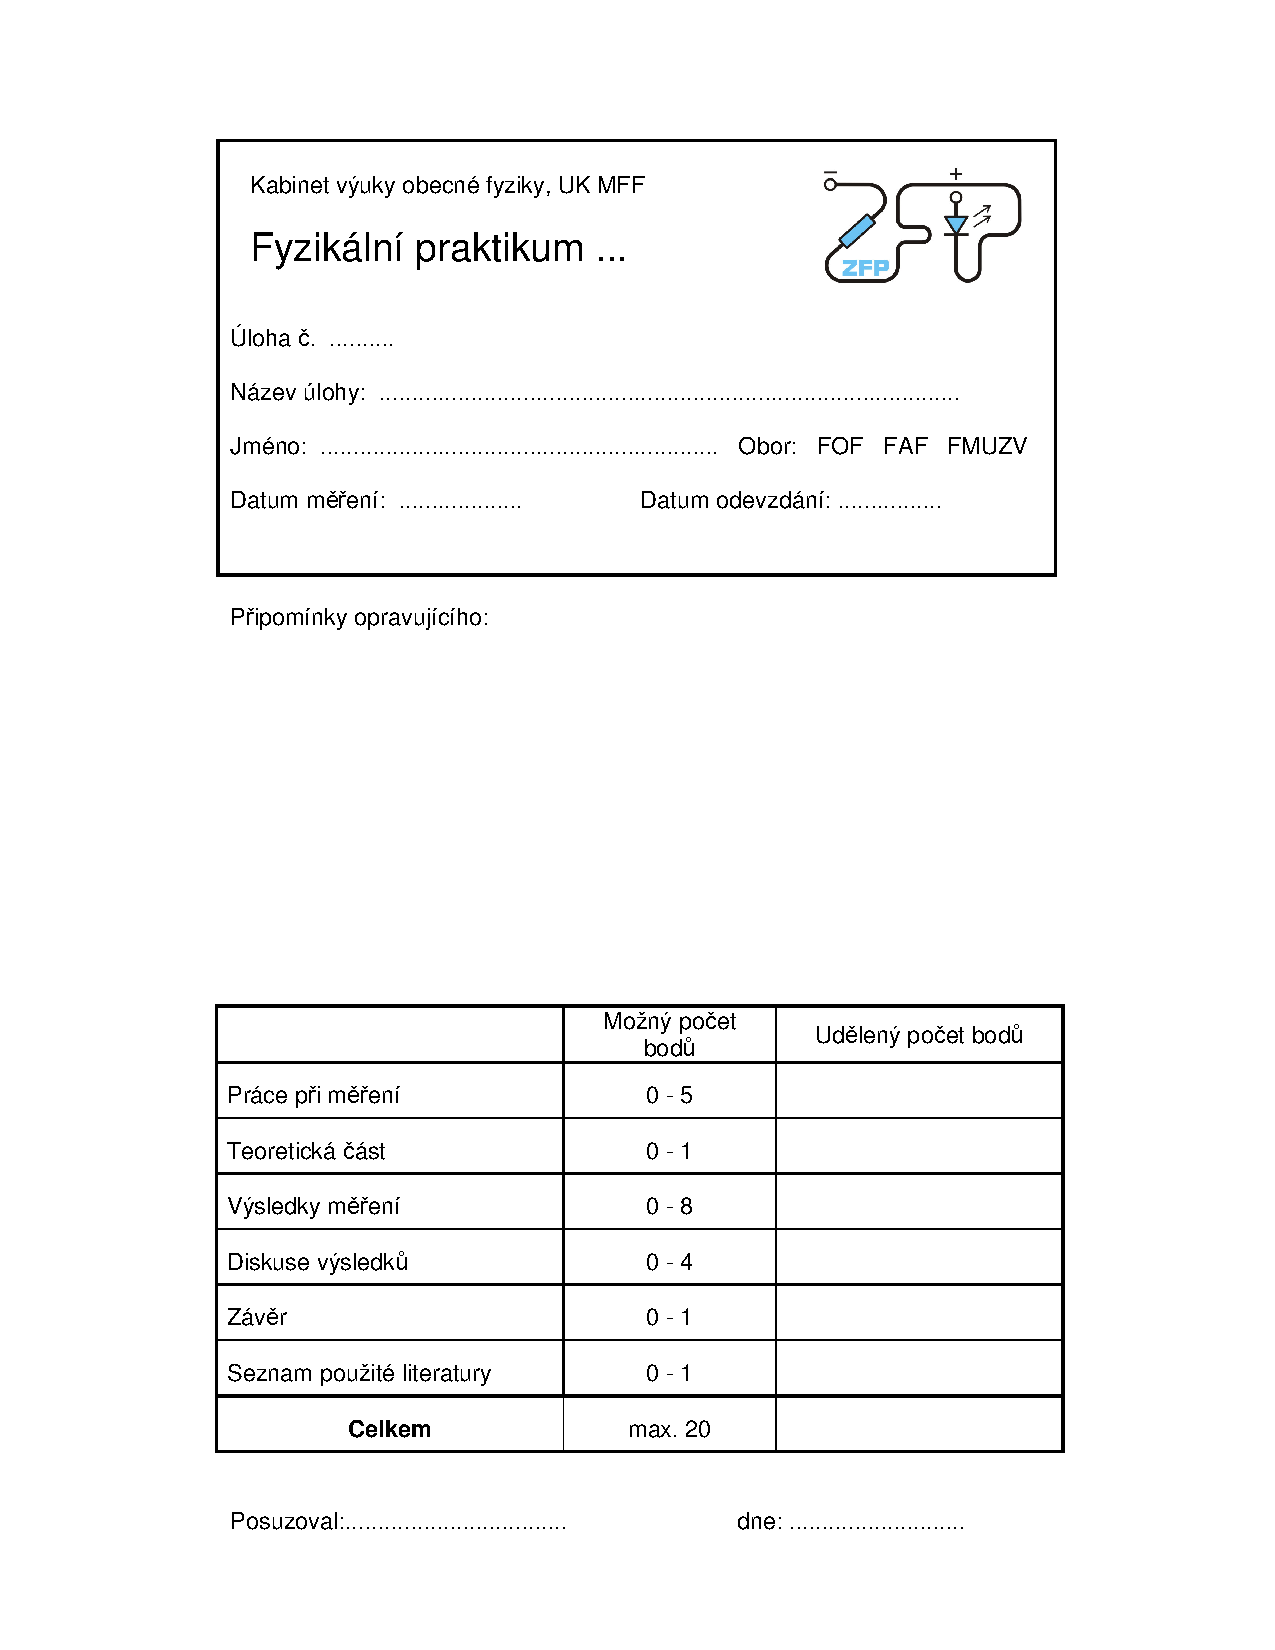
\includepdf[pages={1}]{./graficos/titlelist.pdf}
\end{titlepage}

\section*{Pracovní úkoly}
\begin{enumerate}
\item Prostudujte teoretický popis sestavy a principu HeNe laseru u úlohy (text je v angličtině).
\item Popište princip stimulované emise.
\item Stanovte, pod jakým úhlem jsou umístěna koncová okénka laserové trubice vzhledem k ose rezonátoru a proč?
\item Vysvětlete vliv vzdálenosti zrcadel hemisférického rezonátoru a vliv polohy výbojové trubice v rezonátoru na výkon laseru (případně ověřte měřením).
\item Změřte relativní výkon laseru v závislosti na velikosti proudu procházejícího výbojovou trubicí (POZOR: MAXIMÁLNÍ hodnota proudu je 6,5 mA!!!).
\item Proměřte některé parametry laserového svazku (např. profil svazku, vlnová délka, divergence, stupeň polarizace).

\end{enumerate}

\nocite{skripta}
%Teoretická část
\section*{Teoretická část}

Profil svazku budeme měřit štěrbinovým detektorem s posuvným šroubem. Rozložení intenzity proložíme Gaussovou funkcí tvaru $f(x)=A\cdot \exp(-(x-\mu)^2/2\sigma^2)$.

Vlnovou délku budeme měřit pomocí difrakční mřížky.
Pokud má difrakční mřížka mřížkovou konstantu $a$, stínítko umístíme do vzdálenosti $L$ od mřížky a na stínítku naměříme vzdálenost nultého a prvního maxima $S$, potom vlnová délka laseru je
\begin{equation} \label{e:vlnovadelka}
\lambda = \frac{a}{\sqrt{1+\left(\frac{L}{S}\right)^2}} \,.
\end{equation}

Rozbíhavost svazku charakterizujeme divergencí \cite{div}
\begin{equation} \label{e:div}
d=\frac{D-D_0}{s} \,,
\end{equation}
kde $D$ je průměr svazku ve vzdálenosti $s$ a $D_0$ je průměr svazku u výstupního otvoru laseru.

Stupeň polarizace definujeme vztahem
\begin{equation} \label{e:pol}
Q=\frac{\left|I_{max} - I_{min}\right|}{\left|I_{max}-I_{min}\right|} \,,
\end{equation}
kde $I_{max}$ je maximální intenzita po průchodu polarizátorem a $I_{min}$ je minimální.

\subsection*{HeNe laser}
Stimolavaná emise je jev, při kterém foton dopadající na částici stimuluje přechod excitovaného elektronu do základního stavu, což má za následek vyzáření dalšího fotonu se stejnými vlastnostmi. Aby se stimolavené emise dalo využít k zesílení intenzity světla, je nutná \emph{inverzní populace}, tedy aby více elektronů bylo v excitovaném stavu než v základním stavu. V HeNe laseru se k dosažení inverze využívá proud procházející výbojovou trubicí.

Z obou stran výbojové trubice jsou umístěny zrcadla resonátoru, které zajišťují, aby fotony procházeli trubicí vícekrát a mohlo udržitelně docházet ke stimulované emisi.

Okénka na koncích laserové trubice jsou skloněné vzhledem k optické ose o Brewsterův úhel, aby docházelo k co možná nejmenšímu odrazu. To má za následek, že světlo vycházející z laseru je lineárně polarizované.

%Výsledky měření
\section*{Výsledky měření}

%Diskuze výsledků
\section*{Diskuze}

%Závěr
\section*{Závěr}


\printbibliography[title={Seznam použité literatury}]

\end{document}